%%%%%%%%%%%%%%%%%%%%%%%%%%%%%%%%%%%%%%%%%%%%%%%%%%%%%%%%%%%%%%%%%%%%%%%%
%   LaTeX source code to approximate a NIST Technical report
%	Instructions for authors: tinyurl.com/techpubsnist 
%	DOI watermark will be added on final PDF
% 	Developed by K. Miller, kmm5@nist.gov 
%	Last updated: 22-January-2021
%%%%%%%%%%%%%%%%%%%%%%%%%%%%%%%%%%%%%%%%%%%%%%%%%%%%%%%%%%%%%%%%%%%
\documentclass[12pt]{article}
\usepackage{amsmath}
\usepackage{amsfonts}   % if you want the fonts
\usepackage{amssymb}    % if you want extra symbols
\usepackage{graphicx}   % need for figures
\usepackage{xcolor}
\usepackage{caption}
\usepackage{bm}
\usepackage{secdot}	
\usepackage{listings}	
\usepackage{mathptmx}
\usepackage{float}
\usepackage[utf8]{inputenc}
\usepackage{textcomp}
\usepackage[hang,flushmargin,bottom]{footmisc} % footnote format
\setlength{\parindent}{0pt}

% colori per il codice

\definecolor{codegreen}{rgb}{0,0.6,0}
\definecolor{codegray}{rgb}{0.5,0.5,0.5}
\definecolor{codepurple}{rgb}{0.58,0,0.82}
\definecolor{backcolour}{rgb}{0.95,0.95,0.92}

\lstdefinestyle{mystyle}{
    backgroundcolor=\color{backcolour},   
    commentstyle=\color{codegreen},
    keywordstyle=\color{magenta},
    numberstyle=\tiny\color{codegray},
    stringstyle=\color{codepurple},
    basicstyle=\ttfamily\footnotesize,
    breakatwhitespace=false,         
    breaklines=true,                 
    captionpos=b,                    
    keepspaces=true,                 
    numbers=left,                    
    numbersep=5pt,                  
    showspaces=false,                
    showstringspaces=false,
    showtabs=false,                  
    tabsize=2
}

\lstset{style=mystyle}

\usepackage{titlesec}
\titleformat{\section}{\normalsize\bfseries}{\thesection.}{1em}{}	% required for heading numbering style
\titleformat*{\subsection}{\normalsize\bfseries}

\usepackage{tocloft}	% change typeset, titles, and format list of appendices/figures/tables
\renewcommand{\cftdot}{}	
\renewcommand{\contentsname}{Table of Contents}
\renewcommand{\cftpartleader}{\cftdotfill{\cftdotsep}} % for parts
\renewcommand{\cftsecleader}{\cftdotfill{\cftdotsep}}
\renewcommand\cftbeforesecskip{\setlength{4pt}{}}
\addtolength{\cftfignumwidth}{1em}
\renewcommand{\cftfigpresnum}{\figurename\ }
\addtolength{\cfttabnumwidth}{1em}
\renewcommand{\cfttabpresnum}{\tablename\ }
\setlength{\cfttabindent}{0in}    %% adjust as you like
\setlength{\cftfigindent}{0in} 

\usepackage{enumitem}         % to control spacing between bullets/numbered lists

% \usepackage[numbers,sort&compress]{natbib} % format bibliography 
% \renewcommand{\bibsection}{}
% \setlength{\bibsep}{20.0pt}

\usepackage[hidelinks]{hyperref}
\hypersetup{
	colorlinks = true,
urlcolor ={blue},
citecolor = {.},
linkcolor = {.},
anchorcolor = {.},
filecolor = {.},
menucolor = {.},
runcolor = {.}
pdftitle={},%%put title here to auto-fill properties of the PDF
pdfsubject={},%%put abstract here
pdfauthor={}, %%put author list here
pdfkeywords={} %%put keywords here
}
\urlstyle{same}

\usepackage{epstopdf} % converting EPS figure files to PDF

\usepackage{fancyhdr, lastpage}	% formatting document, calculating number of pages, formatting headers
\setlength{\topmargin}{-0.5in}
\setlength{\headheight}{39pt}
\setlength{\oddsidemargin}{0.25in}
\setlength{\evensidemargin}{0.25in}
\setlength{\textwidth}{6.0in}
\setlength{\textheight}{8.5in}

\usepackage{caption} % required for Figure labels
\captionsetup{font=small,labelfont=bf,figurename=Fig.,labelsep=period,justification=raggedright} 

%%%%%%%%%%% !!!!!! REQUIRED - FILL OUT METADATA HERE !!!!!!!! %%%%%%%%%%%%%%
%  	Report Number - fill in Report Number sent to you (see info below)
%   DOI Statement - fill in DOI sent to you 
%   Month Year - fill in Month and Year of Publication
%%%%%%%%%%%%%%%%%%%%%%%%%%%%%%%%%%%%%%%%%%%%%%%%%%%%%%%%%%%%%%%%%%%%%%%%%%%%%%%%%%%%%%
\newcommand{\pubnumber}{1500-XX}
\newcommand{\DOI}{https://doi.org/10.6028/NIST.SP.1500-XX}
\newcommand{\monthyear}{Month Year}
%%%%%%%%%%%%%%%%%%%%%%%%%%%%%%%%%%%%%%%%%%%%%%%%%%%%%%%%%%%%%%%%%%%%
%   	BEGIN DOCUMENT 
%%%%%%%%%%%%%%%%%%%%%%%%%%%%%%%%%%%%%%%%%%%%%%%%%%%%%%%%%%%%%%%%%%%%
\begin{document}
\urlstyle{rm} % Format style of \url   

%%%%%%%%%%%%%%%%%%%%%%%%%%%%%%%%%%%%%%%%%%%%%%%%%%%%%%%%%%%%%%%%%%%%
%   Cover Page is REQUIRED and must contain the information 
%	displayed here, at a minimum. Additional artwork may be included 
%	(e.g., official project/conference logo, etc.).
%	Pub Number automated based on metadata
%%%%%%%%%%%%%%%%%%%%%%%%%%%%%%%%%%%%%%%%%%%%%%%%%%%%%%%%%%%%%%%%%%%%
\begin{titlepage}
    \begin{flushright}
        %%%%%%%%%%%%%%%%%%%%%%%%%%%%%%%%%%%%%%%%%%%%%%%%%%%%%%%%%%%%%%%%%%%%
        % 	Automated based on metadata - delete if not applicable
        %%%%%%%%%%%%%%%%%%%%%%%%%%%%%%%%%%%%%%%%%%%%%%%%%%%%%%%%%%%%%%%%%%%%
        \LARGE{\textbf{Molecular Simulations Report}}\\
        \vfill
        %%%%%%%%%%%%%%%%%%%%%%%%%%%%%%%%%%%%%%%%%%%%%%%%%%%%%%%%%%%%%%%%%%%%
        %	Title 
        %%%%%%%%%%%%%%%%%%%%%%%%%%%%%%%%%%%%%%%%%%%%%%%%%%%%%%%%%%%%%%%%%%%%
        \Huge{\textbf{Comparative analysis of water structure for HIV-1 Reverse transcriptase in complex with DMP-266 (Efavirenz)}}\\
        \vfill
        %%%%%%%%%%%%%%%%%%%%%%%%%%%%%%%%%%%%%%%%%%%%%%%%%%%%%%%%%%%%%%%%%%%%
        %	Authors - add complete list of authors, affiliations will be 
        %   added on title page
        %%%%%%%%%%%%%%%%%%%%%%%%%%%%%%%%%%%%%%%%%%%%%%%%%%%%%%%%%%%%%%%%%%%%
        \large Conforto Filippo - 2021856\\

        \vfill


        
\includegraphics[width=0.3\linewidth]{logo.png}\\


    \end{flushright}
\end{titlepage}

\begin{center}
    \begin{abstract}
        The combination of Efavirenz with the HIV Reverse transcriptase has a very important role in designing of anti-HIV therapies. The inhibitive role of EFZ was infact tested on different molecular complexes, such as \textbf{1fk9}, 1fko, and 1fkp for RT(wild type)-efavirenz,
        RT(K103N)-efavirenz, and RT(K103N)-nevirapine, respectively \cite{Ren2000}. The following work has the goal to analyze the behaviour of one of these complexes (\textbf{1fk9}) in a water solution, with a focus on the water distribution around the active site of each configuration. To carry out this work molecular dynamics techniques were used, along with model preparation tools \cite{Amber} in order to get ready the system at first, and then simulate its behaviour in the desired solution.
        Finally, the simulation produced underwent the analysis phase, through the use of tools such VMD \cite{VMD}, and MDTraj \cite{MDTraj}.
    \end{abstract}
\end{center}

\pagebreak

%%%%%%%%%%%%%%%%%%%%%%%%%%%%%%%%%%%%%%%%%%%%%%%%%%%%%%%%%%%%%%%%%%%%
%   Table of Contents is required
% 	List of Tables & Figures required if more than 5 tables/figures
%%%%%%%%%%%%%%%%%%%%%%%%%%%%%%%%%%%%%%%%%%%%%%%%%%%%%%%%%%%%%%%%%%%%
\begin{center}
    \tableofcontents
\end{center}
\pagebreak
\section{Introduction}

The biological and medical importance of residues as Efavirenz (EFZ) are related to the interaction they have with larger protein complexes such as the HIV-1 reverse transcriptase. Their interaction with the active site of such proteins allows to inhibit the complex's functionality and be useful in anti-HIV therapies \cite{Ren2000}.
The macromolecule discussed in this work is coded as 1fk9 and represents the combination of a wild type reverse transcriptase(K103N)\cite{pmid3040055} and the EFZ residue.

At the structure level the molecular complex is composed by two chains, while EFZ occupies the active site of the structure.
The first chain of the complex(chain A) contains residues from position 588 to 1130 of the original polyprotein (Uniprot P04585), while the second one contains residues with position 588 to 1027. One additional remark to do on the first chain is that it contains a modified residue of cystine (CYS \cite{CYS}), called CSD \cite{CSD}. The presence of Efavirenz \cite{EFZ} will require its specific modelization, along with the CSD one, before being able to do any simulation on the complex's behaviour.
\begin{figure}[H]
    \centering
    a)
    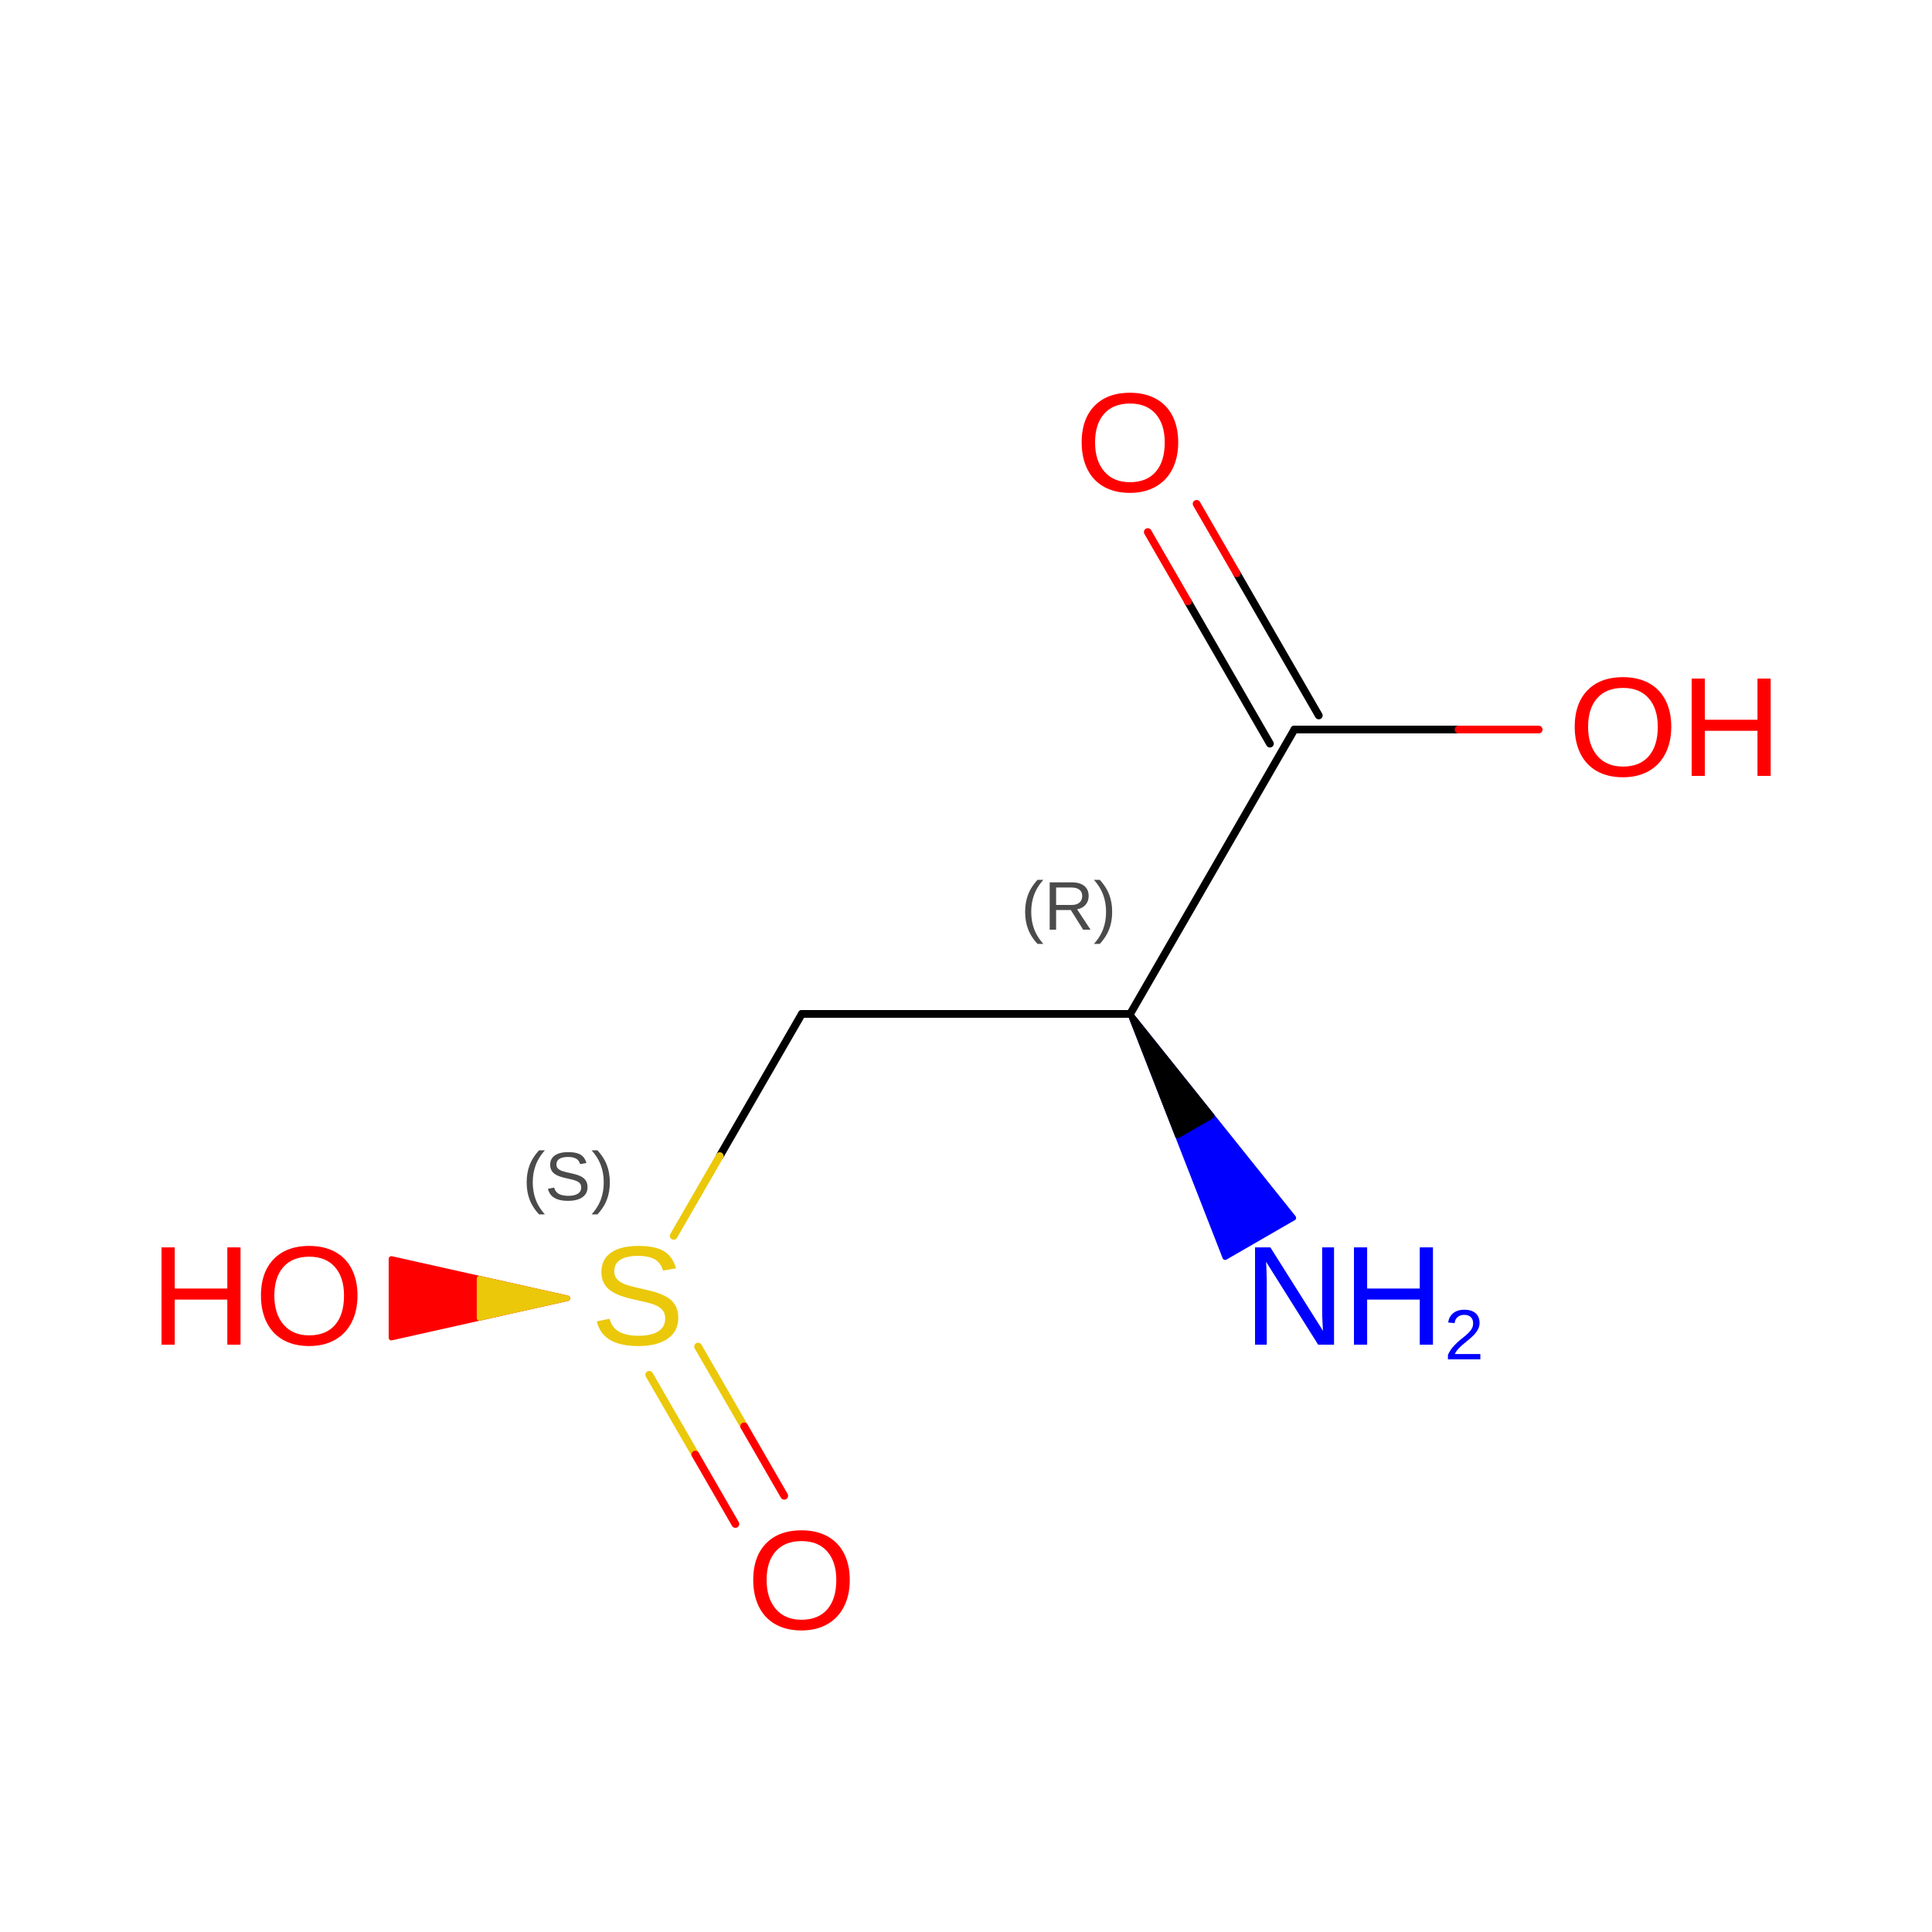
\includegraphics[width=0.4\textwidth]{../figures/CSD.png}
    b)
    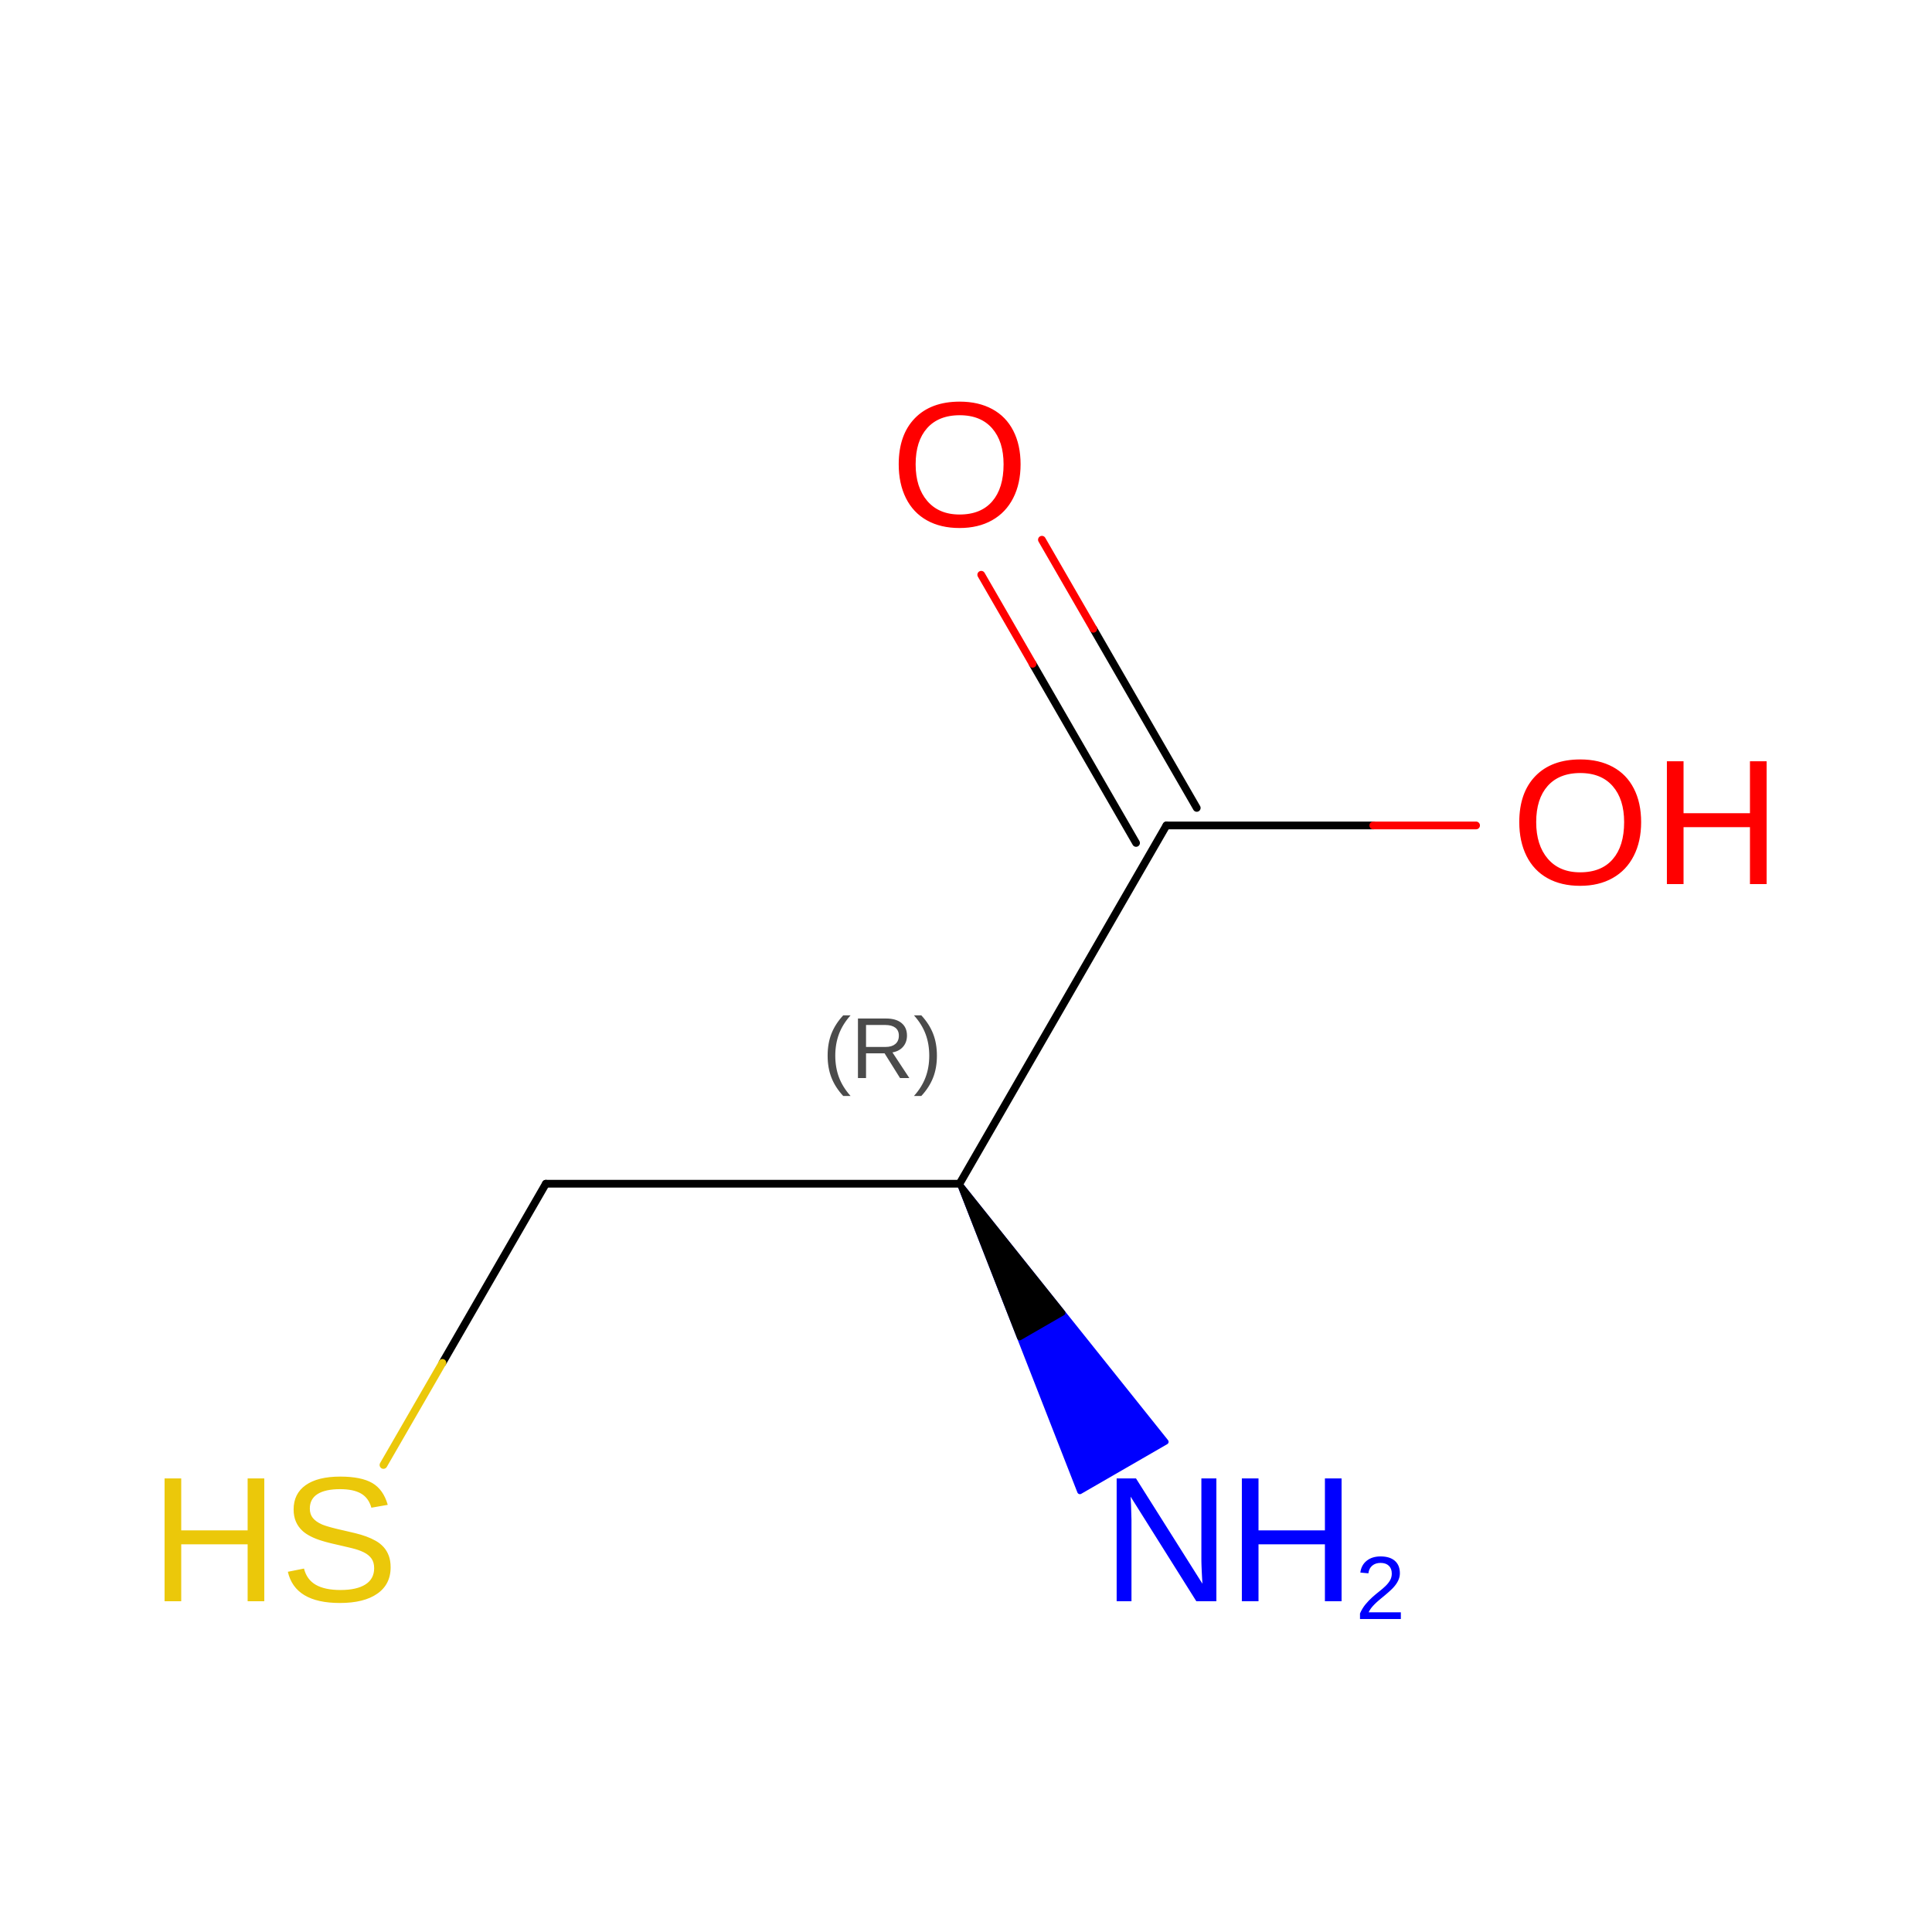
\includegraphics[width=0.4\textwidth]{../figures/CYS.png}
    \caption{CSD (a) and CYS (b).\label{fig:CSDCYS}}
\end{figure}

The CSD residue replaces CYS at the position 867 of original polyprotein sequence, around the middle of the Chain A.

By considering such structure, the main goal of the work was to compare how the molecular complex behaves while constrained in water solution. To do so molecular dynamics methods were applied in order to study the dynamics and the relative distribution of molecules and water.

\section{Methods}
The main applicative used to get the final results was Amber\cite{Amber}, in particular the tools "tleap", "pdb4amber" and "sander". These tools allowed both to prepare the model for the system and executing molecular dynamics simulations of the molecules' behaviour.

The complex's structure was retrieved from the pdb dataset, and contained all the already named chains and residues. The pdb file contained also some HOH elements (water codification), found during the X-Ray Cristallography\cite{SAKABE1991448}.
These water molecules were not taken into account during the elaboration and the successive simulation, since they were replaced later with the pre-equilibrated solvent available in the tip3 library of tleap.
\begin{figure}
    \centering
    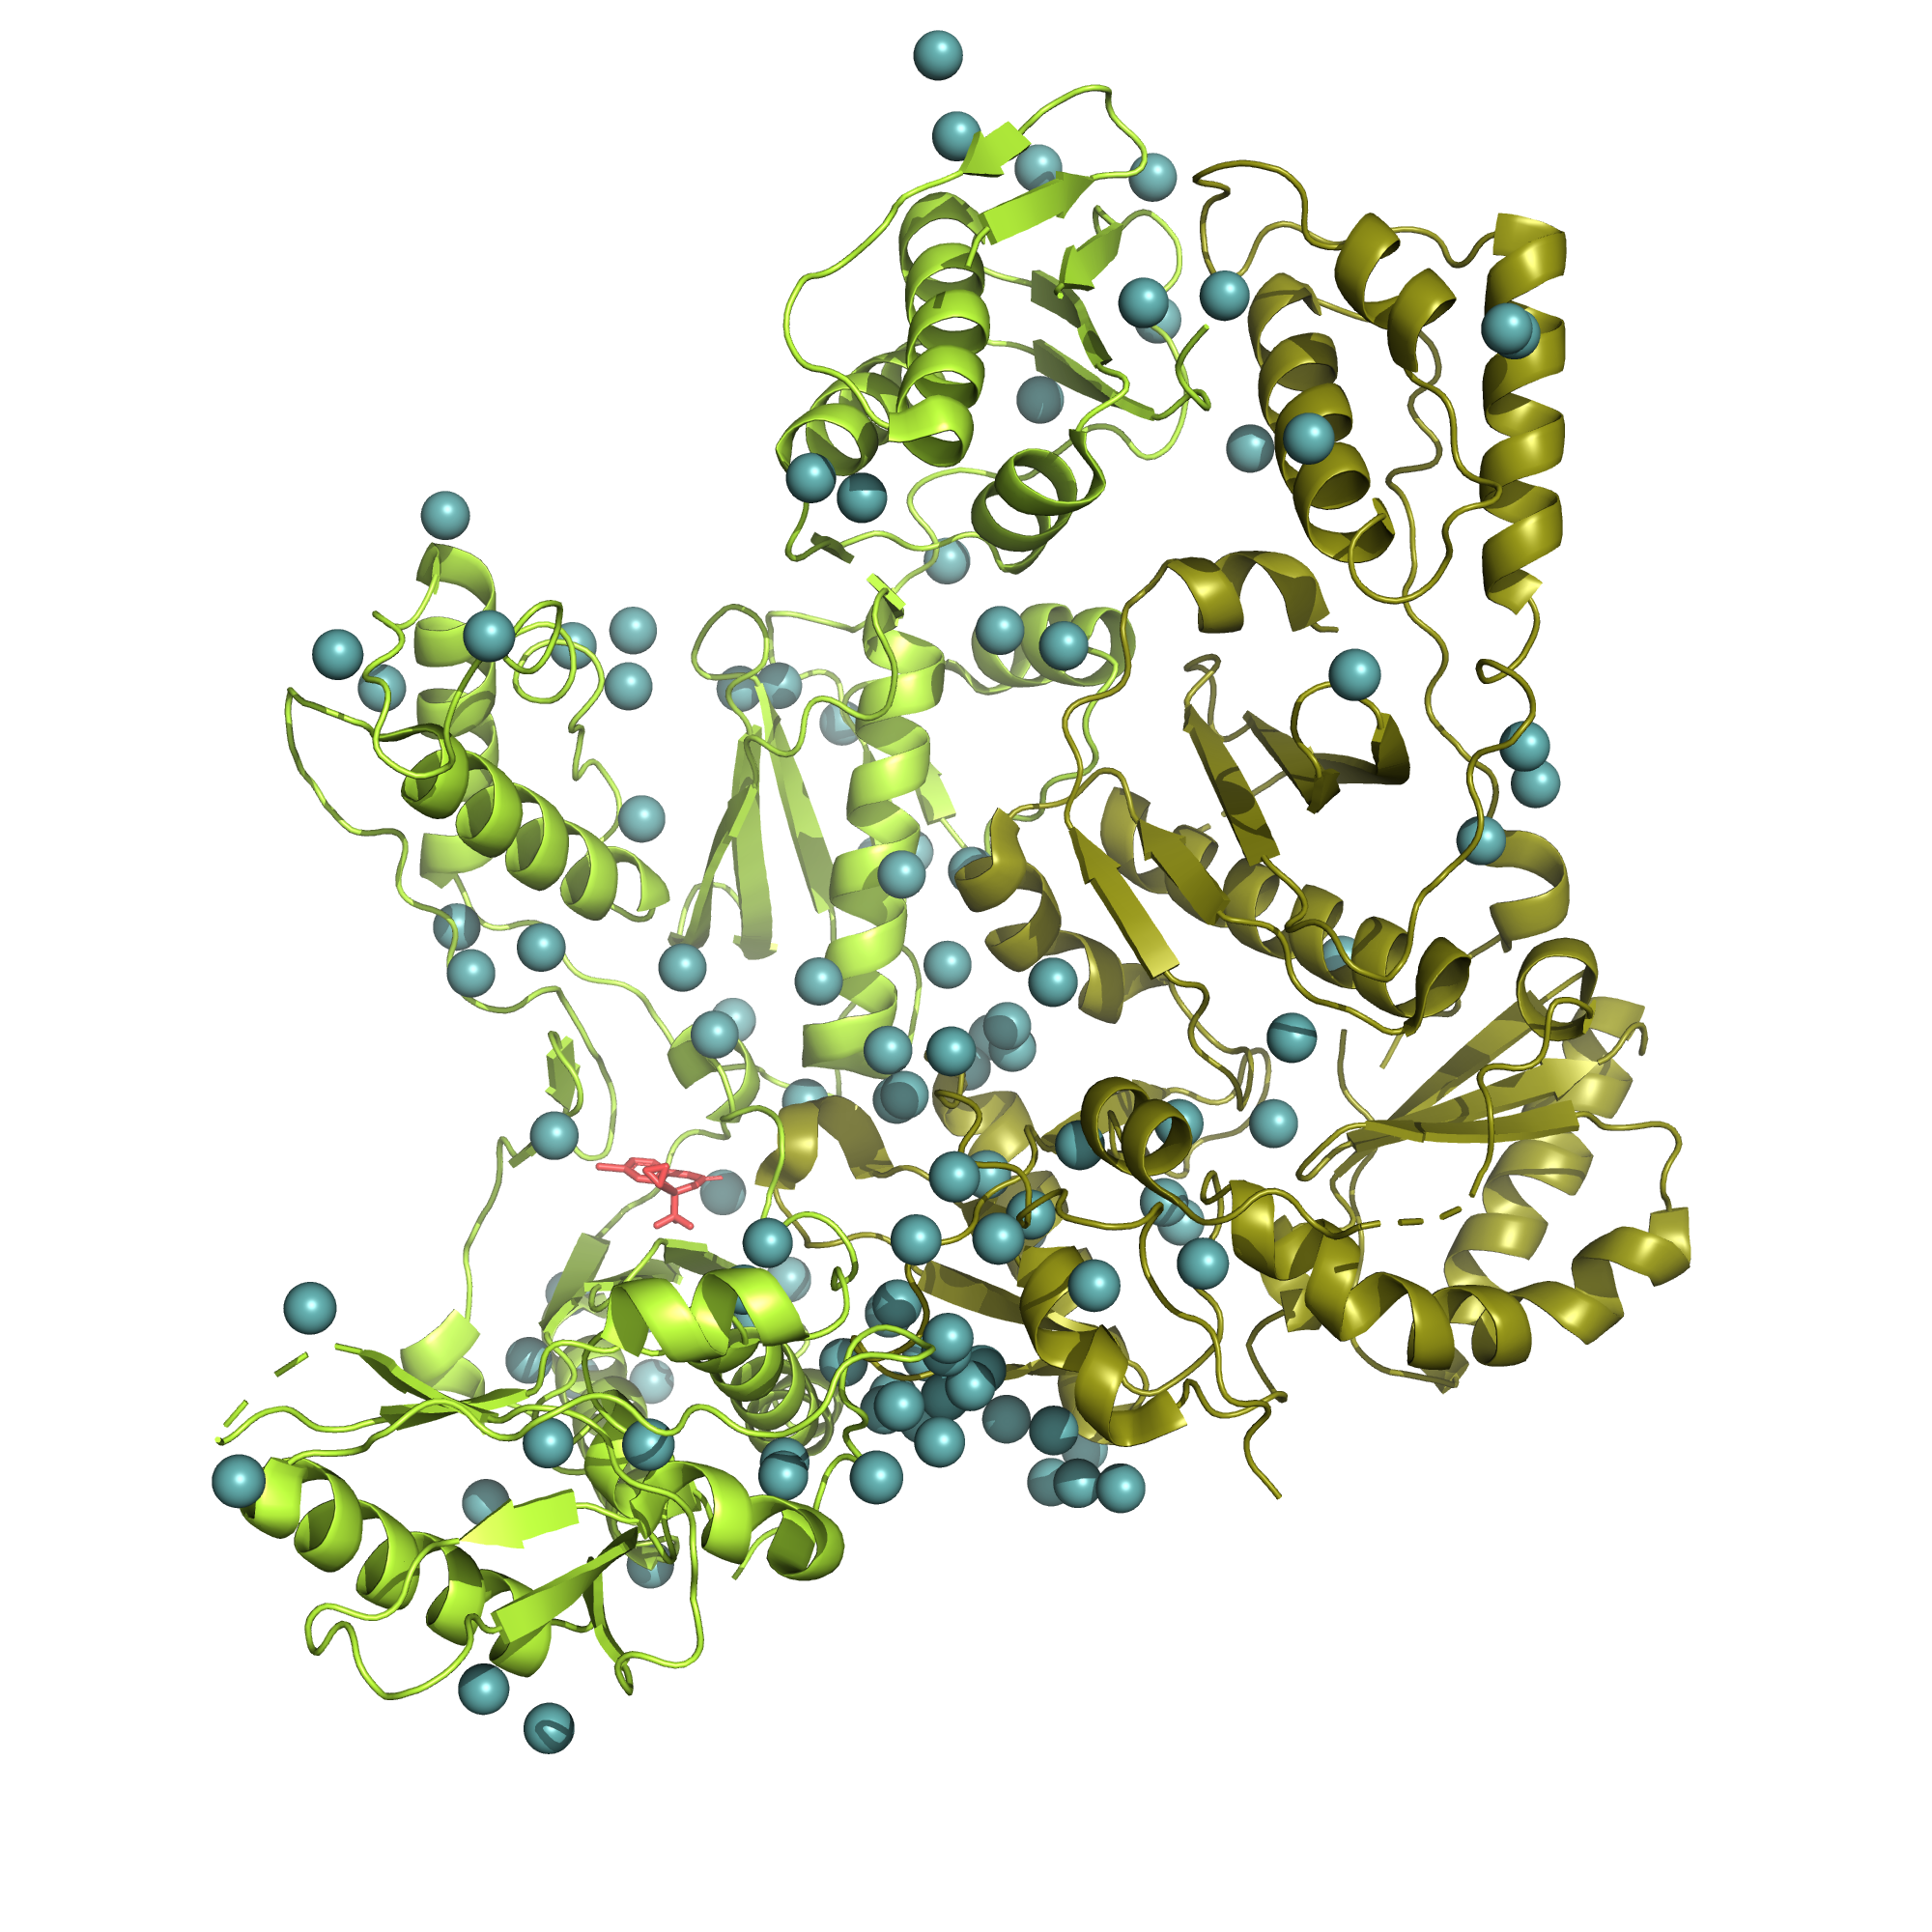
\includegraphics[width=0.5\textwidth]{../figures/water.png}
    \caption{Protein complex, water molecules are represented by the blue beads according to the VdW radius, EFZ is represented in red, Chain A in green, and Chain B in gold. Rendered with \cite[Pymol]{pymol}. \label{fig:total}}
\end{figure}

\subsection{Model preparation}
Since the two residues (CSD and EFZ) were not associated to any force field, the parameters were manually added through model preparation.
Steps followed for such procedures were the same for both the residues, involving these procedures:

\begin{itemize}
    \item Hydrogen addition
    \item Charges computation
    \item General force field (gaff) assignment
\end{itemize}

After these procedures, the final parameters were saved in a .lib file ready to be loaded for the final simulation process.
Given this initial modelization it was decided to study the behaviour of two particular configurations:
\begin{itemize}
    \item Chain A + EFZ
    \item Chain B + EFZ
\end{itemize}
This was done to ease computations by using a smaller set of elements to simulate while having the possibility to study reciprocal behavior of the EFZ residue and the active residues of both the chains. Active residue were individuated before the main elaboration, through Pymol\cite{pymol}, by looking for atoms closer than 4 \AA to EFZ belonging to each chain, visually represented in figure \ref{fig:actres}.

\begin{figure}
    \centering
    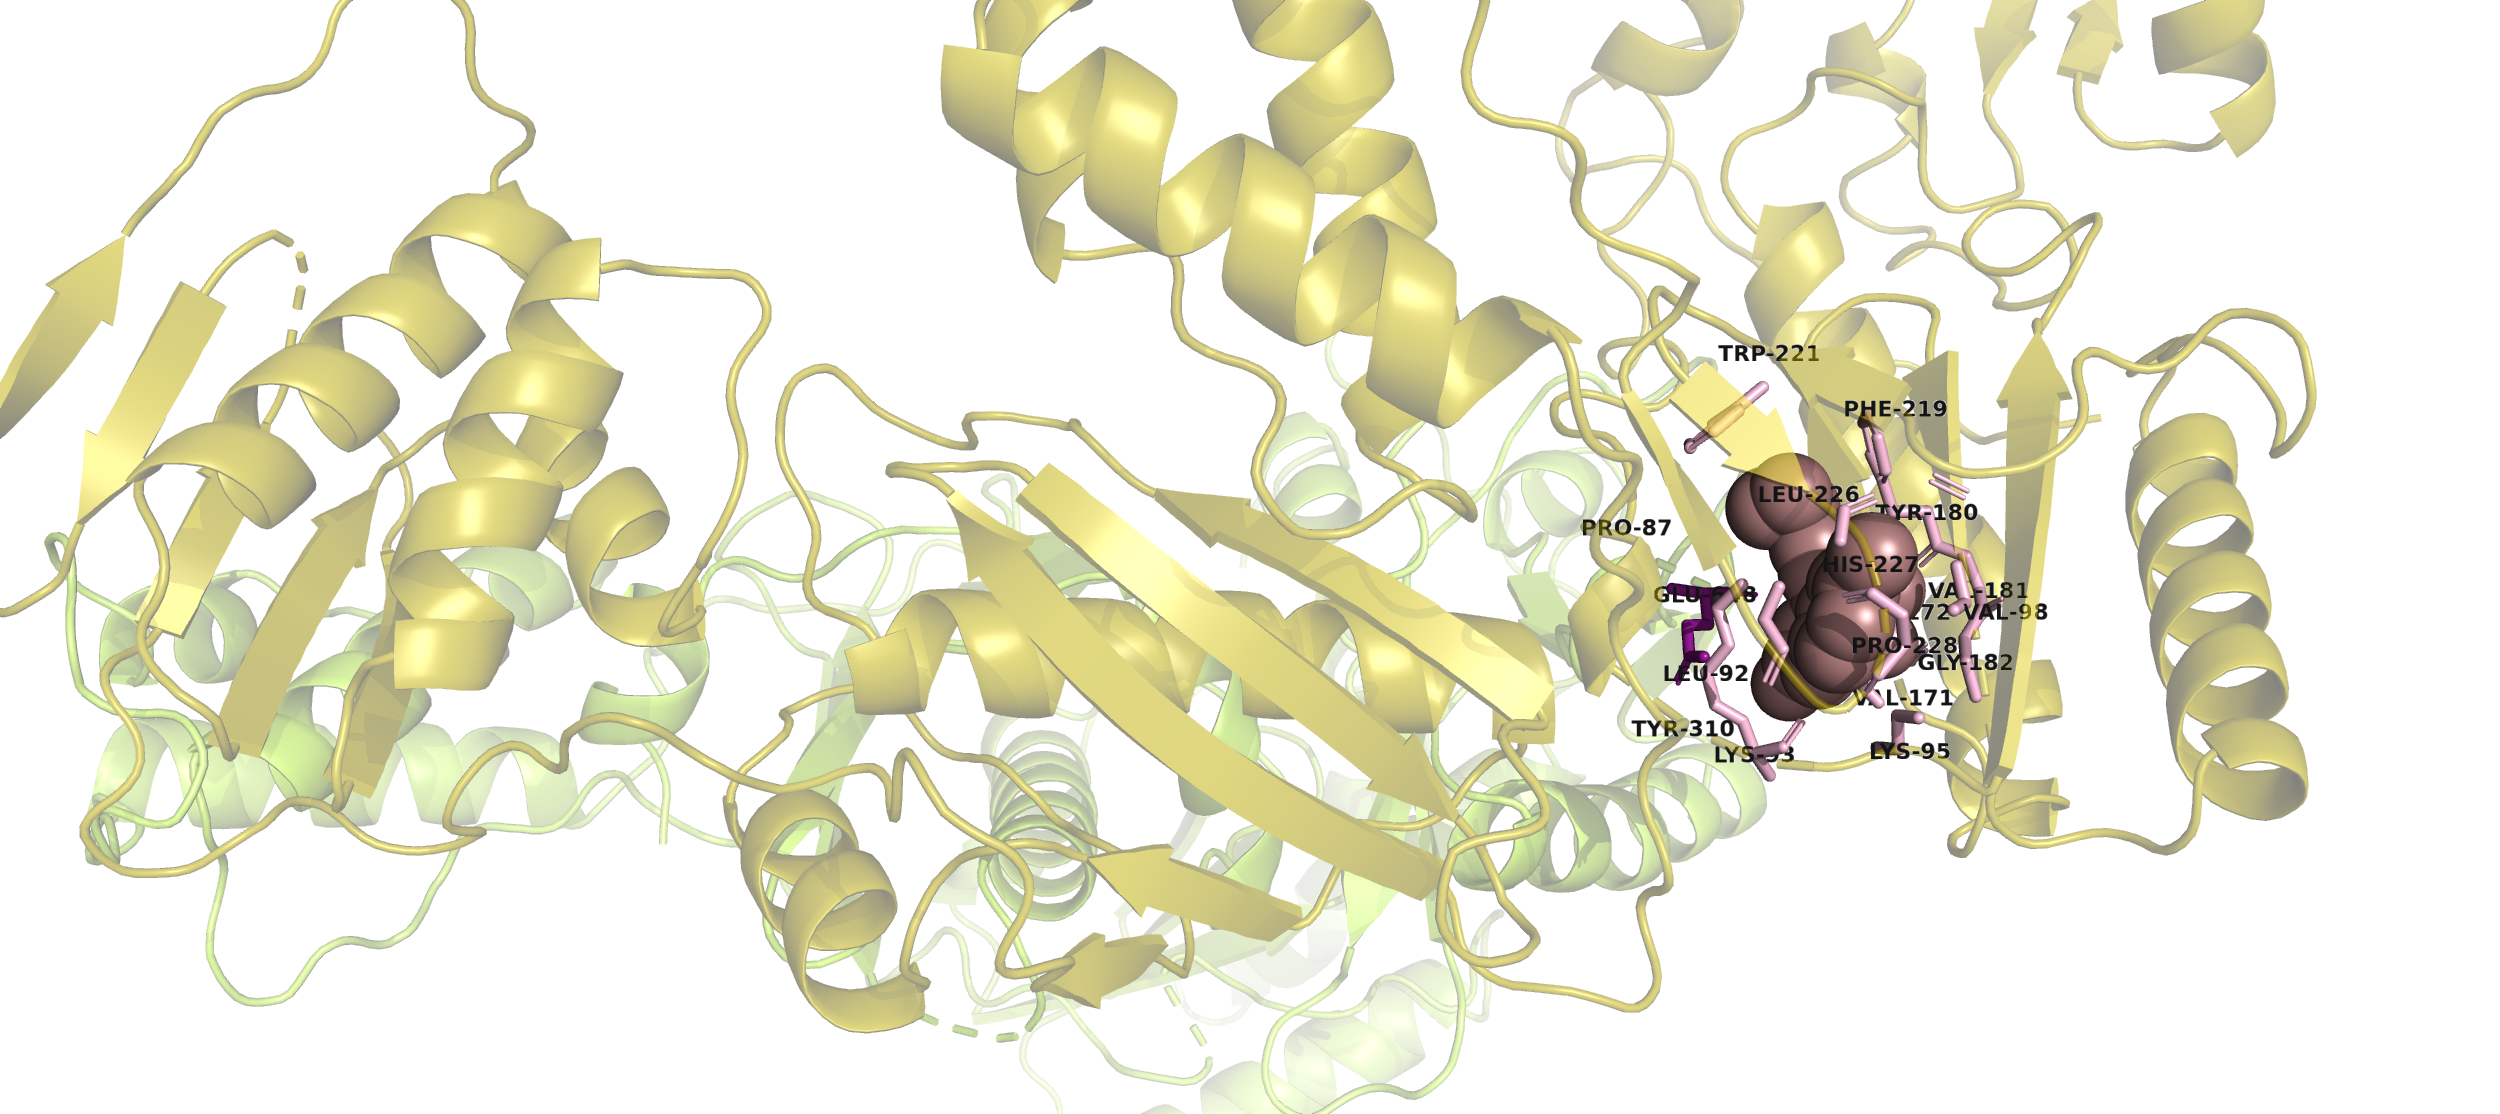
\includegraphics[width=\textwidth]{../figures/act_res.png}
    \caption{Labelled active residues found in the proximity of EFZ (brown beads). Rendered with \cite[Pymol]{pymol} \label{fig:actres}}
\end{figure}
In total were found 15 active residues in the chain A, and a single one in the chain B. These residues will be then considered during
analysis and used as a reference to study the water distribution.

Before any action was taken, the newly-generated pdb files underwent some cleaning through the command "pdb4amber", and were then optimized for a rectangular box through simulaid \cite{simulaid}. After this first optimization it was possible to use tleap, load the pdb file corresponding to each tested configuration and define the force fields using predefined libraries ("ff99SB") and user-defined ones for the CSD and EFZ residues. In this last phase some warnings were raised by tleap concerning improper tension terms, but were considered negligible and so the global model was accepted as generally correct.

\subsection{Solvent addition and minimization}
After having prepared the model for the two sistems to simulate, preequilibrated water was added using "TIP3" library of tleap using a rectangular box filled with water with maximum distance from solvate fixed at 12 \AA. Ions were also added to the system to neutralise the charges, whose sum was equal to +6 in the Chain B + EFZ case, and equal to -2 in the Chain A + EFZ case.
These charges were balanced with respectively by adding 6 Cl- ions in the first case, and 2 Na+ ions in the latter one. Once again some errors were raised by tleap, but were similar to the ones found during the loading phase and then considered ininfluential.

Given this initial configuration it was possible to start a minimization routine using periodic boundary conditions along 2000 iterations with a cut fixed at 15 \AA. This last process allowed to retrieve a stable configuration, moving from starting energies equal to $E=1.5\cdot 10^{13}$ for the Chain A + EFZ case and $E=-1.1\cdot 10^{5}$ for che Chain B + EFZ to respectively energies equal to $E=-3.4\cdot 10^{5}$ and $E=-2.6\cdot 10^{5}$.

\begin{figure}
    \centering
    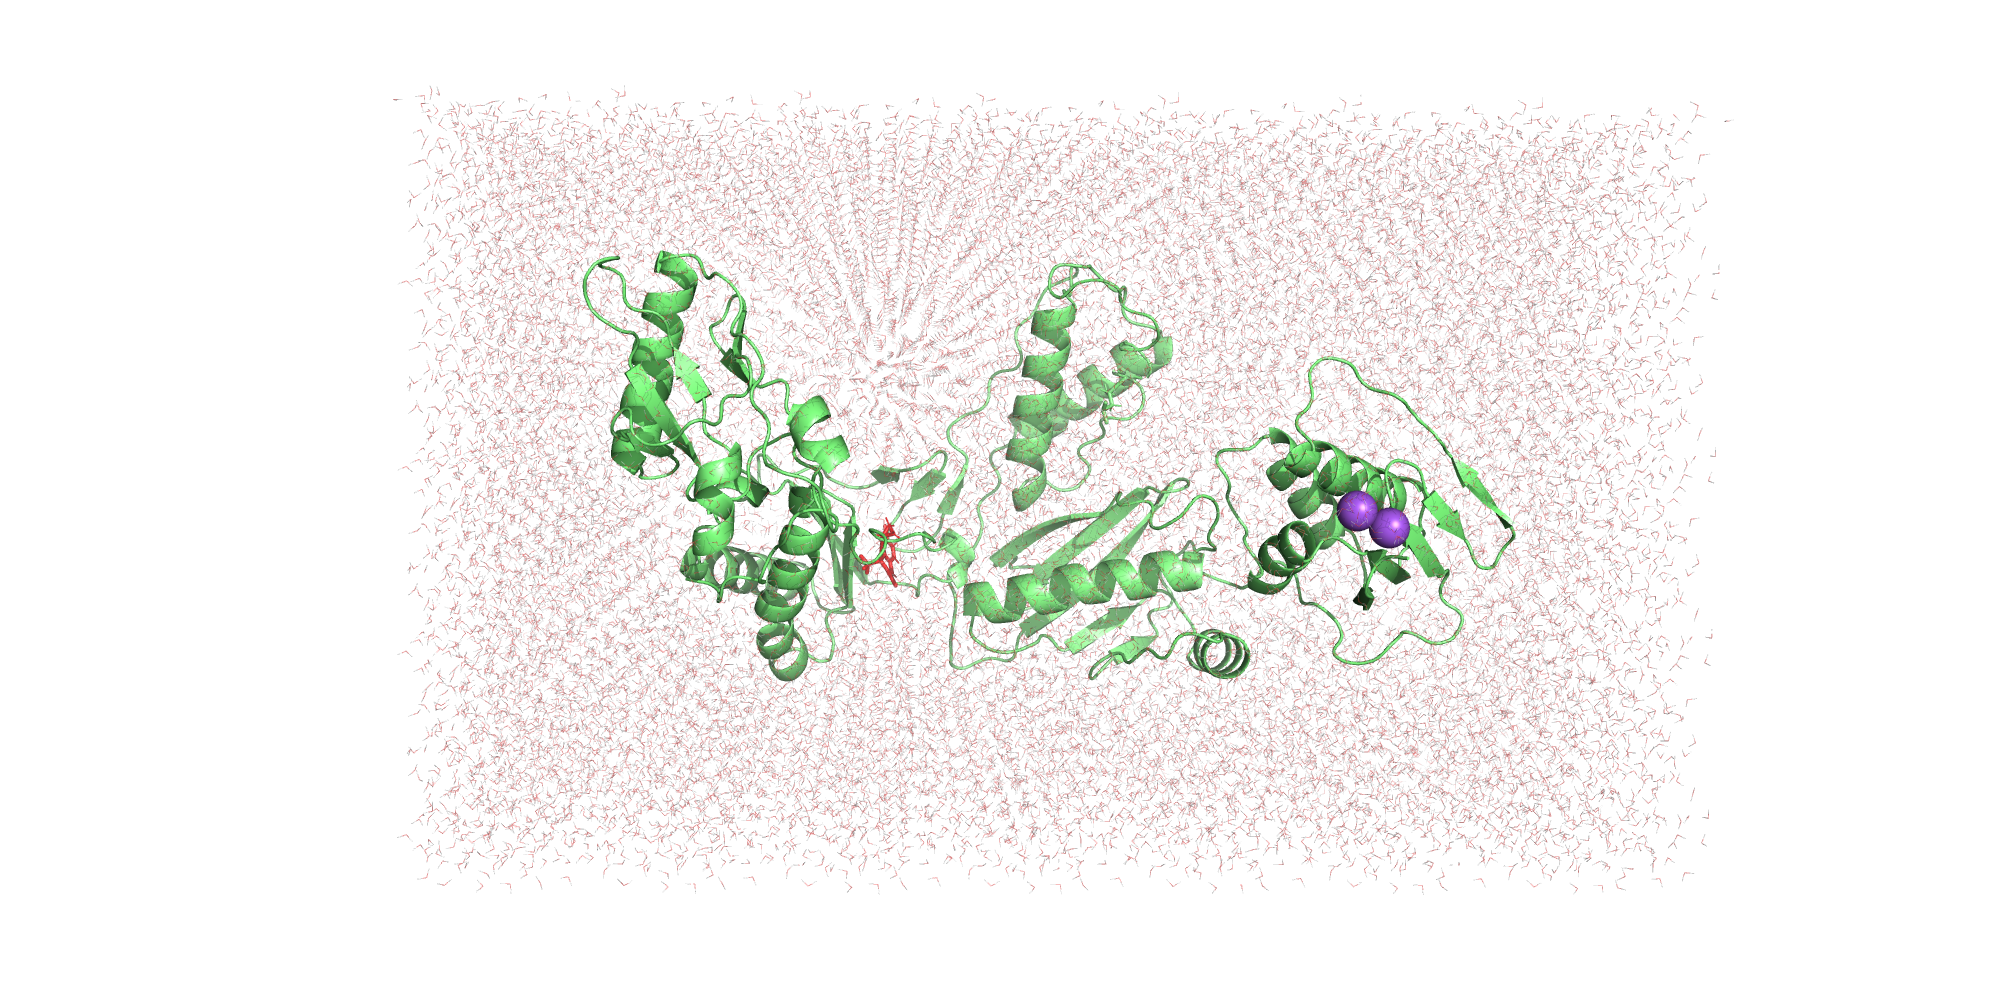
\includegraphics[width=0.8\linewidth, clip, trim= 0 0 0 0]{../figures/chain_a_efz_solv.png}
    \caption{Chain A+ EFZ configuration in solution after minimization. In red can be seen the EFZ residue, while the purple beads represent the Na+ ions. Rendered with \cite[Pymol]{pymol}.\label{fig:chain_a_efz_solv}}
\end{figure}

\begin{figure}
    \centering
    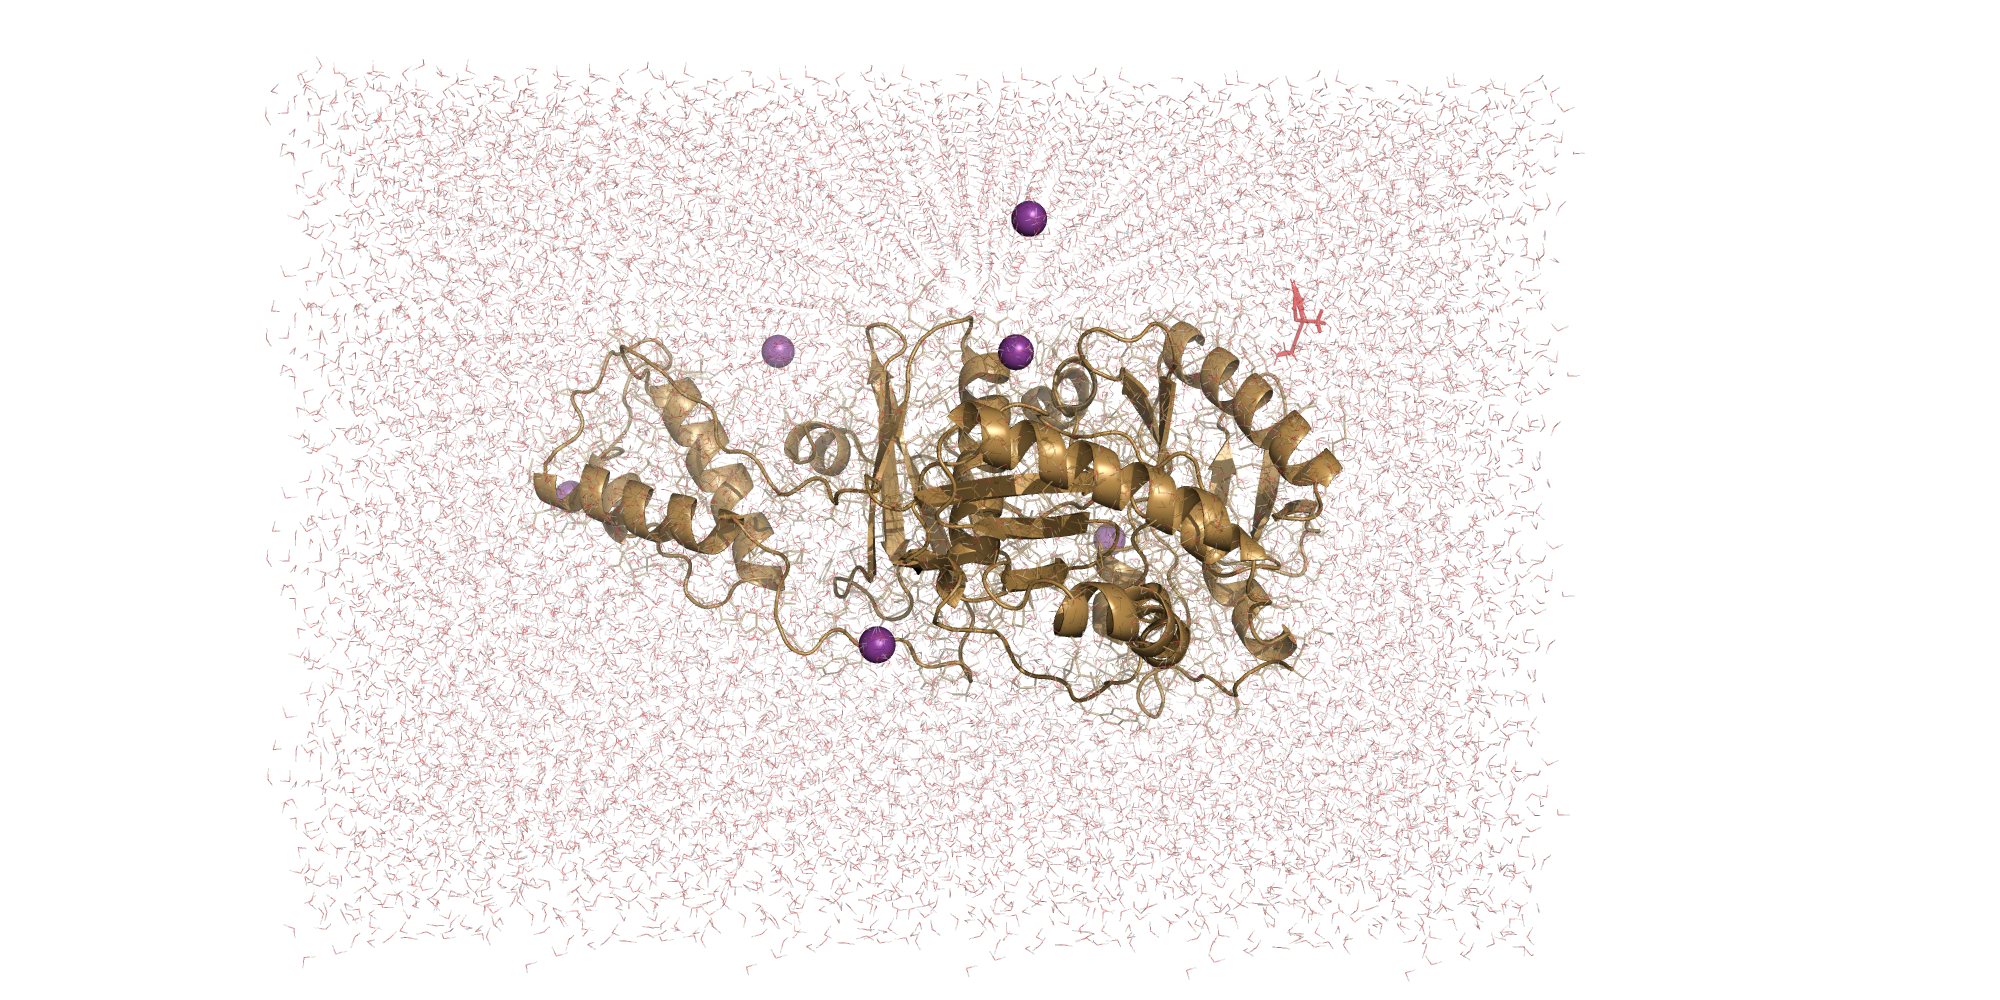
\includegraphics[width=0.8\linewidth, clip, trim= 0 0 0 0]{../figures/chain_b_efz_solv.png}
    \caption{Chain B + EFZ configuration in solution after minimization. In red can be seen the EFZ residue, while the purple beads represent the Cl- ions. Rendered with \cite[Pymol]{pymol}.\label{fig:chain_b_efz_solv}}
\end{figure}

\subsection{Molecular dynamics}
The minimized configuration's atoms don't have any initial speed, that have to be assigned by fixing an initial temperature and extracting them randomly from the Boltzmann distribution. Through a second script, the system, starting from this initial configuration, was heaten up in periodic boundary conditions from an initial temperature of 0 K, to a final temperature of 298 K. This was done in an isothermic and isobaric esemble coded using a Langevin thermostat. Along with these settings the cut was again fixed at 15 \AA, while the hydrogen movement was constrained with a harmonic potential.
The heating procedure was finally carried out in 10000 steps, each one of 2 fs. This allowed in both cases to reach the required temperature without fluctuations larger than a few degrees.


After having heaten up the system it was possible to perform the actual molecular simulation and study the system at a fixed temperature. A simulation with the same settings of the one discussed for the heating was set up, with the temperature fixed at 298 K as before, and run for 10000 iterations.
Again, thanks to the Langevin thermostat it was possible to keep almost fixed the temperature around the required value, with an RMS that was calculated to be around 1 to 2 degrees in both the tests done.

\subsection{Analysis methods}
The main interest of these simulations is to study and discuss the behaviour of water molecules and active residues during the time they are run. To do so two software utilities were used:
\begin{itemize}
    \item VMD\cite{VMD}, to calculate the radial distribution function g(r)
    \item MDTraj\cite{MDTraj}, to study the trajectory of the simulated structure and compute the running coordination number $K(r)$.
\end{itemize}

Both these tools refer to the following formulas:
\begin{equation}
    g(r) = \frac{V}{4\pi r^2 \Delta r N^2}\sum_i n_i(r,\Delta r) \quad n_i = \mathrm{number \, of \, atoms \, in \, the \, \{r,\Delta r\} \, shell}
    \label{eq:gofr}
\end{equation}
\begin{equation}
    K(r) = 4\pi \rho \int_{0}^{r_c} dr \, r^2 g(r) \quad \rho = \mathrm{particle \, density}
    \label{eq:kofr}
\end{equation}

These formulas the were discretized by dividing the radius domain in intervals of length equal to 0.1 \AA, in order to be applied on the simulation's results.

Along with these analyses, were considered also the calculation of RSMD of the global complex and the RSMF of the EFZ residue. The first computation allowed determining how much the protein's residues moves globally from the starting configuration, during the simulation, by computing the mean deviation from the reference structure (the initial one). The latter one instead allowed understanding how much a single atom fluctuated from a reference configuration of a single residue, that in this case will be EFZ.

A final check was also done on the distance between the substrate EFZ from the active site. The active site position was identified in the discussed cases as the center of mass of the active residues for each simulated molecular complex. In the Chain A+EFZ simulation was represented by the average of 15 positions, while for the Chain B+EFZ was directly identified with the single active residue.
\section{Results}

\subsection{Radial distribution function and coordination number}
The first calculation was done to compute the radial distribution function g(r), in order to understand the local distribution of water molecules around the active sites and the EFZ ligand. The calculation was done taking into account the periodic boundary conditions, allowing to calculate over distances much larger than the 12\AA \, of the solvation box.

\begin{figure}
    \centering
    \includegraphics[width=\textwidth, clip, trim= 0 0 600 0]{../figures/a_chain_act.pdf}
    \caption{Radial distribution function g(r) and running coordination number K(r) of water around active sites for the configuration Chain A + EFZ. g(r) in dark blue, while K(r) in light blue.\label{fig:gofr_chain_a_efz_1}}
\end{figure}

\begin{figure}
    \centering
    \includegraphics[width=\textwidth, clip, trim= 600 0 0 0]{../figures/a_chain_act.pdf}
    \caption{Radial distribution function g(r) and running coordination number K(r) of water around active sites for the configuration Chain A + EFZ. g(r) in dark blue, while K(r) in light blue.\label{fig:gofr_chain_a_efz_2}}
\end{figure}
Only a few residues show a significative local structure, for example the residue 93 in figure \ref{fig:gofr_chain_a_efz_1}, showing a hydration cell around
2 \AA, or the residue 98, in figure \ref{fig:gofr_chain_a_efz_2}, with two hydration shells at 2 and 3 \AA. A single shell can be also found in figure \ref{fig:gofr_chain_a_efz_2} for the residue 95, but also for residue 227.
Around residues like 310,180 and 172 it is possible to observe similar structures, with smaller peaks, idicating less dense shells. The other residues have in general more repulsive behaviours, including EFZ, with a shape increasing continuosly with distance.

\begin{figure}[H]
    \centering
    \includegraphics[width=\textwidth]{../figures/b_chain_act.pdf}
    \caption{Radial distribution function g(r) and running coordination number K(r) of water around active sites for the configuration Chain B + EFZ. g(r) in dark blue, while K(r) in light blue.\label{fig:gofr_chain_b_efz}}
\end{figure}

In the second tested configuration (figure \ref{fig:gofr_chain_b_efz}) results were very similar, with the residue EFZ having a less repulsive behaviour, but the same continuos increase with distance. Residue 129 instead has a clear hydration cells at 2 \AA.

For the coordination numbers the only difference between different residues is related to the repulsivity, that influences in different ways the slope of the line.

\subsection{RMSF and RMSD}
\begin{figure}[H]
    \centering
    \includegraphics[width=\textwidth]{../figures/rmsd.pdf}
    \caption{Global RSMD for the Chain A + EFZ case (a) and the Chain B + EFZ case (b).\label{fig:rmsd}}
\end{figure}
In both cases, as can be seen from figure \ref{fig:rmsd}, the complex RMSD remseble a global movement that seems to move the structure away from the original configuration. However, the small scale at which this phenomenon happens allows to conclude that the complex is in general stable and such fluctuations can be easily explained with the high temperature at which the simulation is done. The increasing trend of RMSD could be eventually verified in longer simulations to see if the value decreases at any time.

\begin{figure}[H]
    \centering
    \includegraphics[width=\textwidth]{../figures/rmsf_efz.pdf}
    \caption{RSMF of the EFZ residue for the Chain A + EFZ case (a) and the Chain B + EFZ case (b).\label{fig:rmsf}}
\end{figure}

The RMSF in figure \ref{fig:rmsf} of EFZ shows instead how the of EFZ behaves during the simulation, confirming that the ones from 20 to 25 (all hydrogens) are the ones which moves the most, together with atom 0(Chlorine),17(Carbon N°11) and 18(Carbon N°12) in the first case and 17(Carbon N°11),18(Carbon N°12) in the second one. This result makes sense given that the Chloride atoms represent an extremity of the aromatic ring, while the two carbons can be found inside a triangular formation of three carbon atoms with apparently a large movement freedom.

\begin{figure}
    \centering
    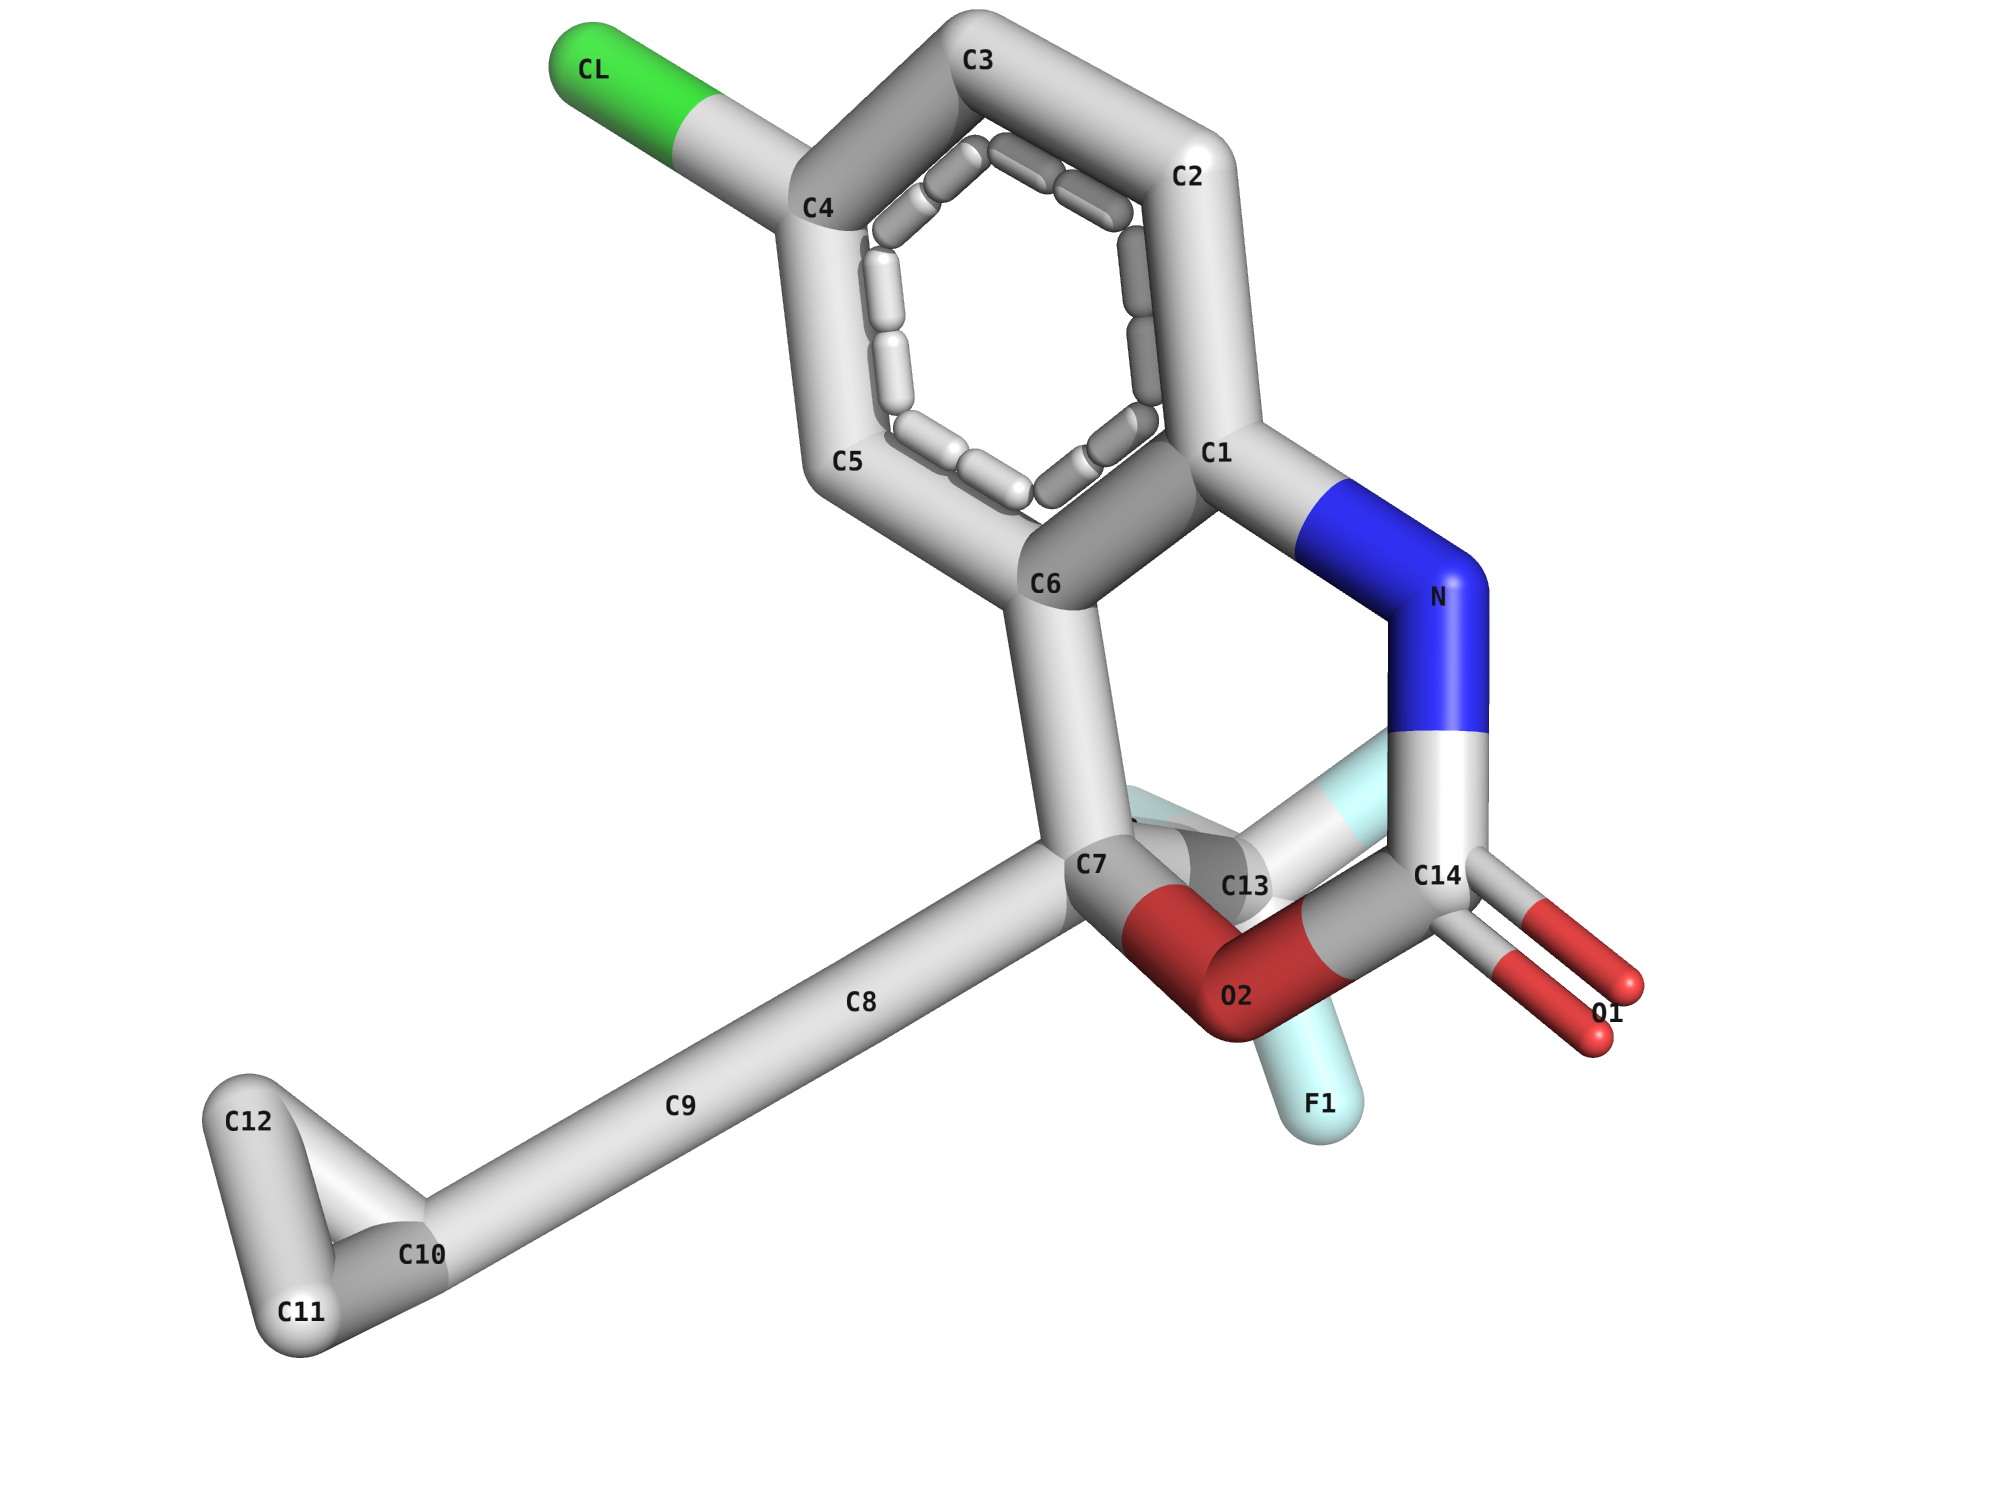
\includegraphics[width=0.4\textwidth]{../figures/efz.png}
    \caption{EFZ ligand. Rendered with \cite[Pymol]{pymol}.\label{fig:efz}}
\end{figure}

\subsection{Substrate movement with respect to active site}

\begin{figure}[H]
    \centering
    \includegraphics[width=\textwidth]{../figures/dis_chain_act.pdf}
    \caption{EFZ distance from the active site for the Chain A + EFZ case (a) and the Chain B + EFZ case (b).\label{fig:dist}}
\end{figure}

In figure \ref{fig:dist}, the position of EFZ's atoms with respect to the active site was calculated along the simulation. For the first tested configuration (Chain A + EFZ) it can be seen that the distance is in average stable, with some bouncing between a minimum and a maximum value, probably associated to temperature.

In the second configuration the trend is instead different, with a slower movement towards the active residue, that allows the substrate to reach a minimum distance near the simulation end. This last configuration may not be a stable one, since, as it can be noticed, in next steps the residues begins again to move away from the active residue. Conclusions on such topic could be eventually taken only with longer simulations.
\section{Conclusions}
The simulation carried out with the molecular dynamics techniques allowed to take an  experimental structure and merge it with theoretical potentials to get a complete model of the complex to simulate. Through Amber\cite{Amber} it was also possible to put the system in a preequilibrated box of water and try to replicate experimental condition with the use of periodic boundary conditions. This new system was ready to be heaten up and then simulated for a long period in order to understand its behaviour.

The analysis returned a lot of insights on the behavior of water around the simulated configurations. Thanks to the calculation of g(r)[\ref{eq:gofr}] and K(r)[\ref{eq:kofr}] it was possible to study the actual distribution of water molecules around active sites. In particular the g(r) computation allowed to appreciate the presence of hydration shells around some residues, while observing hydrofobicity in other ones. 

The analysis of RMSD of the full protein instead allowed understanding if and how the simulated complex was able to stabilize around a configuration or not, while the RMSF calculation for EFZ improved the understanding of the residue mobility along the simulation, and in particular what atoms moved the most from the original configuration.

Finally, the distance of EFZ from the active site allowed understanding how much the substrate actually moved in a water solution, with respect to the active site, unveiling clear trends, such as for the Chain B + EFZ configuration, in which the residue came closer to the main chain. 

Further measurements could eventually test the same complexes using MonteCarlo techniques to improve the accuracy of measurements and analytics.
\section{Source code}
All the code used during the project computations and its outputs can be found in the following GitHub \href{https://github.com/Confizolo/PoDProjects}{repository}, in the "MS" subdirectory.
\bibliographystyle{plain} % We choose the "plain" reference style
\bibliography{bibl} % Entries are in the refs.bib file

\end{document}
